
\section{Features Generation}\label{sec:evaluation-features-generation}
As session files, containing mouse positions of users, are inputted to the back-end server, the features generator is deployed to extract features sets in realtime. Doing so is costly on a server. Since the average number of polled mouse positions is about 125 times per second, and sessions last for numerous minutes, session files contain an average of tens of thousands of lines. Every line of the session files are used and fed through the features generator. Generation of the 6 outputted feature vectors, velocity, horizontal velocity, vertical velocity, acceleration, jerk, and theta, require input of each line of a session file. The computational cost of the features generation step is very high.

Evaluation of the features generator consisted of a few different architectures. For the sake of comparison and additional test data, a Windows and Linux machine were used to run programs written in Python and Golang. With the intention of viewing results and keeping the research process simple, the features generator was originally written in Python. As the program's robustness increased, results were viewed, and runtimes increased, the decision to create the features generator in Golang was influenced by runtime optimization. Since this detection scheme is intended to be run in realtime on a server, and the computation cost of the features generation step is intensive, converting to and parallelizing with Golang seemed like a reasonable investment.

\begin{table}[h!]
    \centering
    \begin{tabular}{ |c|c|c|c|c|c| }
        \hline
        \textbf{system} & \textbf{cores} & \textbf{clock{\_}speed} & \textbf{memory} & \textbf{cpu{\_}desc} & \textbf{exec{\_}env} \\
        \hline
        Open{\_}SUSE & 4 & 1.6GHz & 8GB-DDR4 & 8th-Gen-i5 & native-Bash \\
        Windows{\_}10 & 4 & 3.4GHz & 12GB-DDR4 & 6th-Gen-i7 & winpty-Bash \\
        \hline
    \end{tabular}
    \caption{Environments used to generate session features}
    {\small \textbf{Both systems use a solid-state hard drive.} Comparison of the different environments used to generate features from the mouse position data inputted from the user's computer. \textit{Each result shown are averages of 3 separate runtimes}}
\end{table}

Below are metrics reflecting the total runtimes of each architecture. The Linux machine is run on an Open{\_}SUSE Tumbleweed Linux instance. A Bash terminal was used to execute the Python and Golang programs. However, the Python runtime results varied drastically on the Windows machine. There is one explanation relating to a "wrapper" program, winpty, that had to be used to invoke the Python interpreter. This wrapper-like program acts as an interface between the underlying Windows operating system and the Bash terminal. Enabling users to run Unix programs, winpty must have an overhead cost when using its interface. As you can see, the runtimes are nearly 3 times the amount of the Linux equivalents. Regardless, all runtimes were most often shorter when run on the Linux machine.

There is a bottleneck in the system design. A Bash script was used to execute the features generator program, which takes one session file as input and outputs 6 feature vectors by writing them to files named with the convention \textit{sessionid} {\_} \textit{userid} {\_} \textit{featurename}.json in a separate directory.

\begin{figure}[!h]
    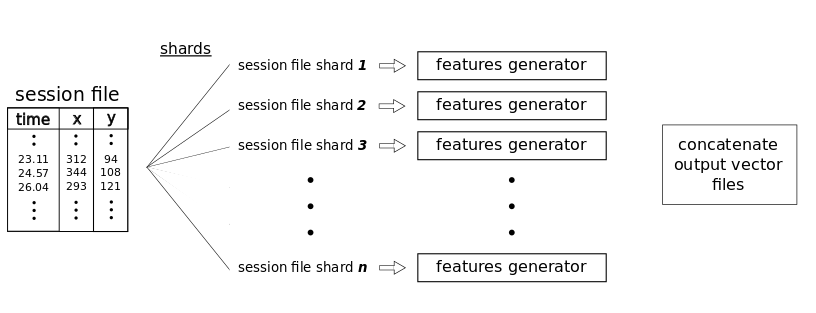
\includegraphics[width=1\columnwidth]{figures/parallelized_features_generator_distributed}
    \caption{Distribution of the parallelized features generator}
    \label{fig:distribution-of-the-parallelize-features-generator}
    {\small The figure at~\ref{fig:parallelization-of-the-features-generator-implementation-version} describes the parallelization of the features generator. This figure displays the sharding and distribution of calculating features from an inputted sessions file.}
\end{figure}

While this Bash script is sufficient in this research on how to differentiate users by clustering, there is one design change that will significantly reduce the runtime of the system. Instead of using a program that sequentially takes input, like this Bash script, a parallelized "master" program is a necessary design decision. Figure~\ref{fig:distribution-of-the-parallelize-features-generator} shows how distribution of the features generation may occur. Although the Golang metrics reflect a parallelized program, which generates the 6 feature vectors in parallel, a master node can be used to take inputted session files and trigger multiple executions of the features generator. Additionally, session files can be split into several "shards" that would reduce the required execution time of each features generator executable. Preferably, this parallelization would be distributed across many Linux boxes equipped with the features generator executable.

\begin{figure}
    \centering
    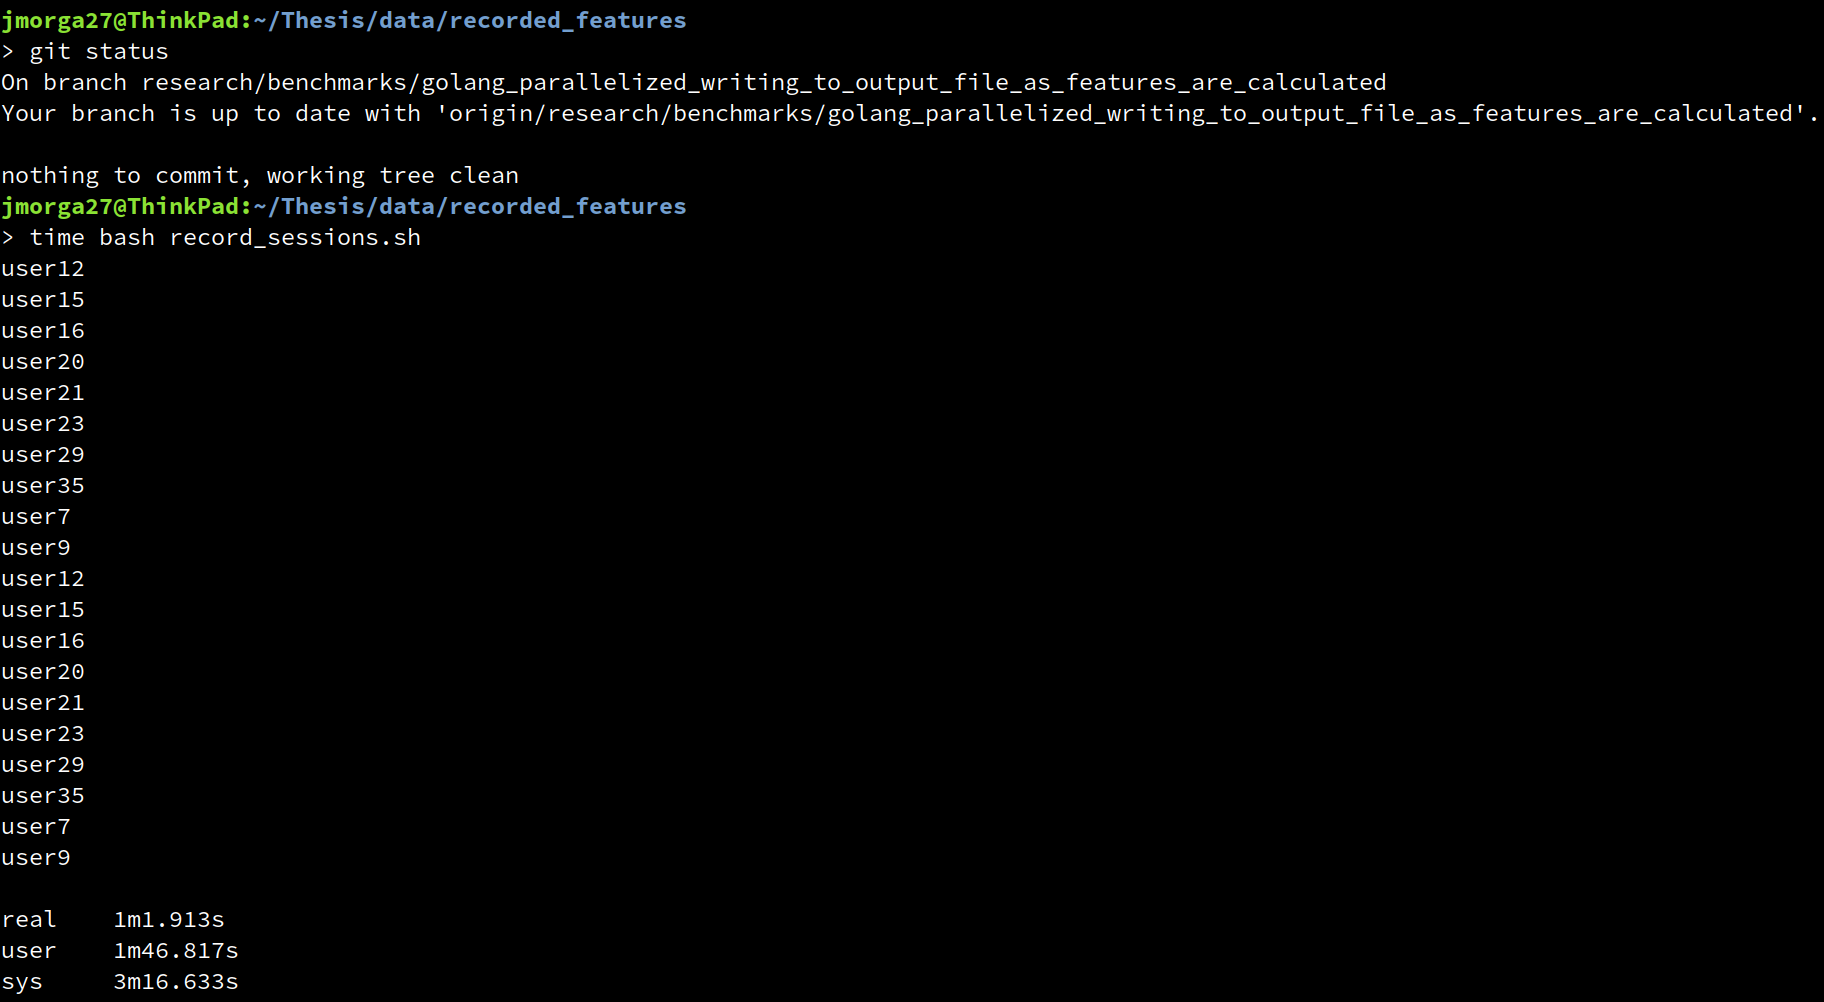
\includegraphics[width=1\columnwidth]{figures/bash_feature_generator_runtime_screenshot_linux}
    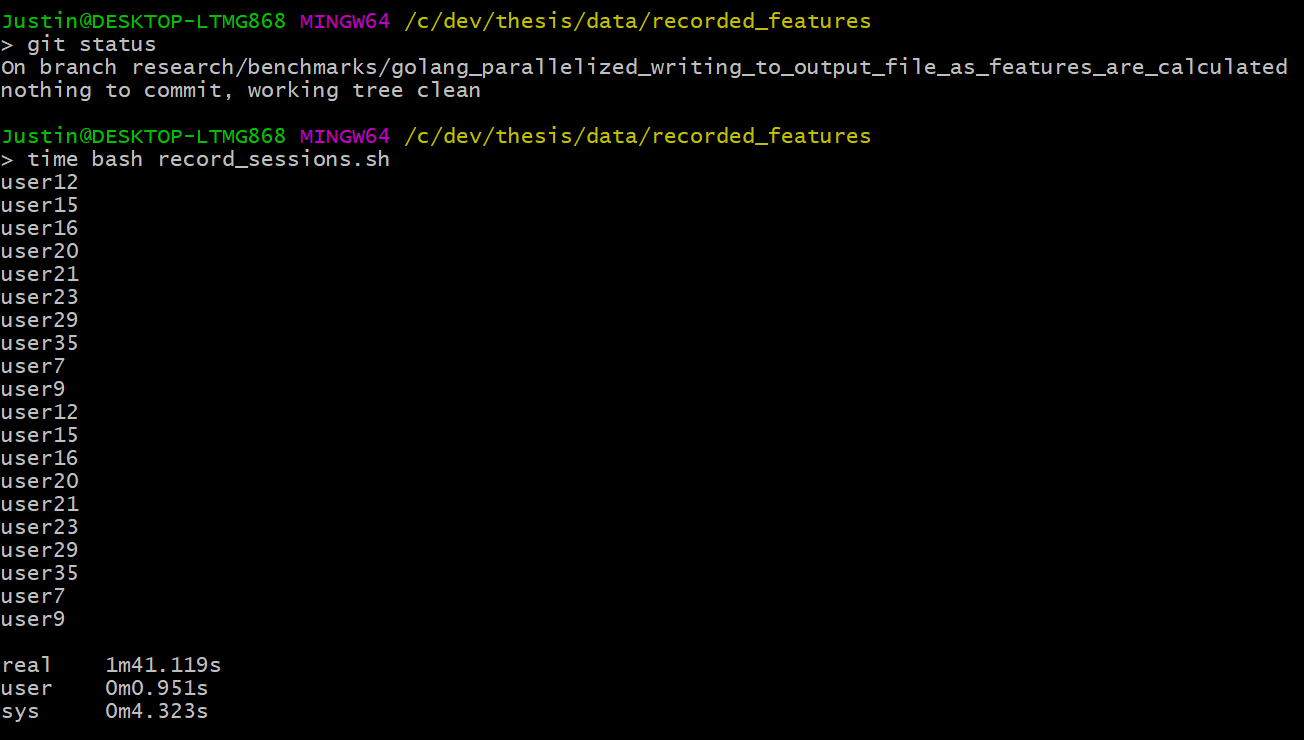
\includegraphics[width=1\columnwidth]{figures/bash_feature_generator_runtime_screenshot_windows}
    \caption{Screen shots of the Bash script running the features generator}
    {\small Both screenshots, Linux (top) and Windows (bottom), include two printouts of the users. This is because the inputted session files consist of a training and testing dataset, per the Balabit dataset~\cite{balabit_dataset}}
    \label{fig:bash-features-generator-runtimes}
\end{figure}

\begin{table}[h!]
    \centering
    \begin{tabular}{ |c|c|c|c|c| }
        \hline
        \textbf{method} & \textbf{lin{\_}go} & \textbf{win{\_}go} & \textbf{lin{\_}py} & \textbf{win{\_}py} \\
        \hline
        list{\_}buf & 1m5s & 1m42s & 3m16s & 11m16s \\
        prealloc{\_}list{\_}buf & 0m36s & 2m25s & 3m31s & 10m52s \\
        file{\_}append & 1m13s & 1m42s & 3m18s & 10m55s \\
        go{\_}seq & 0m46s & 3m4s & -- & -- \\
        \hline
    \end{tabular}
    \caption{Runtimes of different features generation methods}
    {\small A "list" buffer was used for Python execs, while a "slice" was the equivalent buffer used for Golang execs. Python on the Windows system was run through an API, winpty, that enables Bash terminals to run Unix-like programs. This may account for the significantly slower Python runtimes on Windows}
\end{table}

Three different methods, \textit{list or slice buffer}, \textit{preallocated list or slice buffer}, \textit{file append}, and an additional sequential Golang method, were used to compare the different features generator architectures. The list or slice buffer method showed slower runtimes since memory had to be reallocated upon data insertions. By preallocating the memory space, with a given size number, there is no longer a need to reallocate memory for this buffer type. This explains why the preallocated list or slice buffers had a faster average runtime. However, an interesting observation is with runtimes of the Windows preallocated slice buffer and file append methods. Results show that, while using a non-preallocated slice in Golang had the same runtime as the file append method in Golang, the preallocated slice buffer method resulted in slower runtimes. One explaination would be the quality of the solid state hard drives. Thought both systems use a solid state hard drive as their main storage, the Windows system is equipped with an aftermarket SSD. Perhaps the file write speed is quicker with this hard drive, thus decreasing the runtime of the file append method. However, there is uncertainty with this theory.

Of the different methods used, the preallocated slice buffer with Golang method used on the Linux machine showed the best results. This is what prompted the deployment of a non-parallelized, sequential version of the preallocated slice buffer method with Golang was added for comparison. As the results reflect, preallocated slice buffers boast the lowest runtimes in Golang. However, the sequential version of the Golang generator showed poor results on the Windows system. This may be attributed to the slow runtimes of the parallelized preallocated slice buffer method results. An additional explanation could be the method used to obtain the size needed for preallocation. Since the number of lines of the input file is the size used to preallocate the slice buffer, the process of reading the input file may be the culprit. Perhaps there were file system blocks associated with the slower runtimes. Regardless, the optimal architecture for the features generator was the parallelized, preallocated slice buffer method with Golang on the Linux machine.
